\section{Experimental Validation}
\label{sec:experiments}

We validate the Squiggly Line Conjecture through comprehensive experiments across multiple dimensions, architectures, and data distributions.

\subsection{Experimental Setup}

We tested the conjecture across multiple dimensions:
\begin{itemize}
    \item \textbf{Dimensions}: $d \in \{2, 3, 4, 5\}$
    \item \textbf{Network widths}: $w \in \{20, 40, 80\}$
    \item \textbf{Depths}: $L \in \{1, 2, 3, 4\}$
    \item \textbf{Data distributions}: Uniform, Gaussian, Clusters, Manifold
    \item \textbf{Dataset size}: $n = 1000$ points
\end{itemize}

Networks used fully connected feedforward architectures with ReLU activations and random Gaussian initialization: $w_{ij} \sim \mathcal{N}(0, \sigma^2/\sqrt{\text{fan-in}})$.

\begin{figure}[ht]
\vskip 0.2in
\begin{center}
\centerline{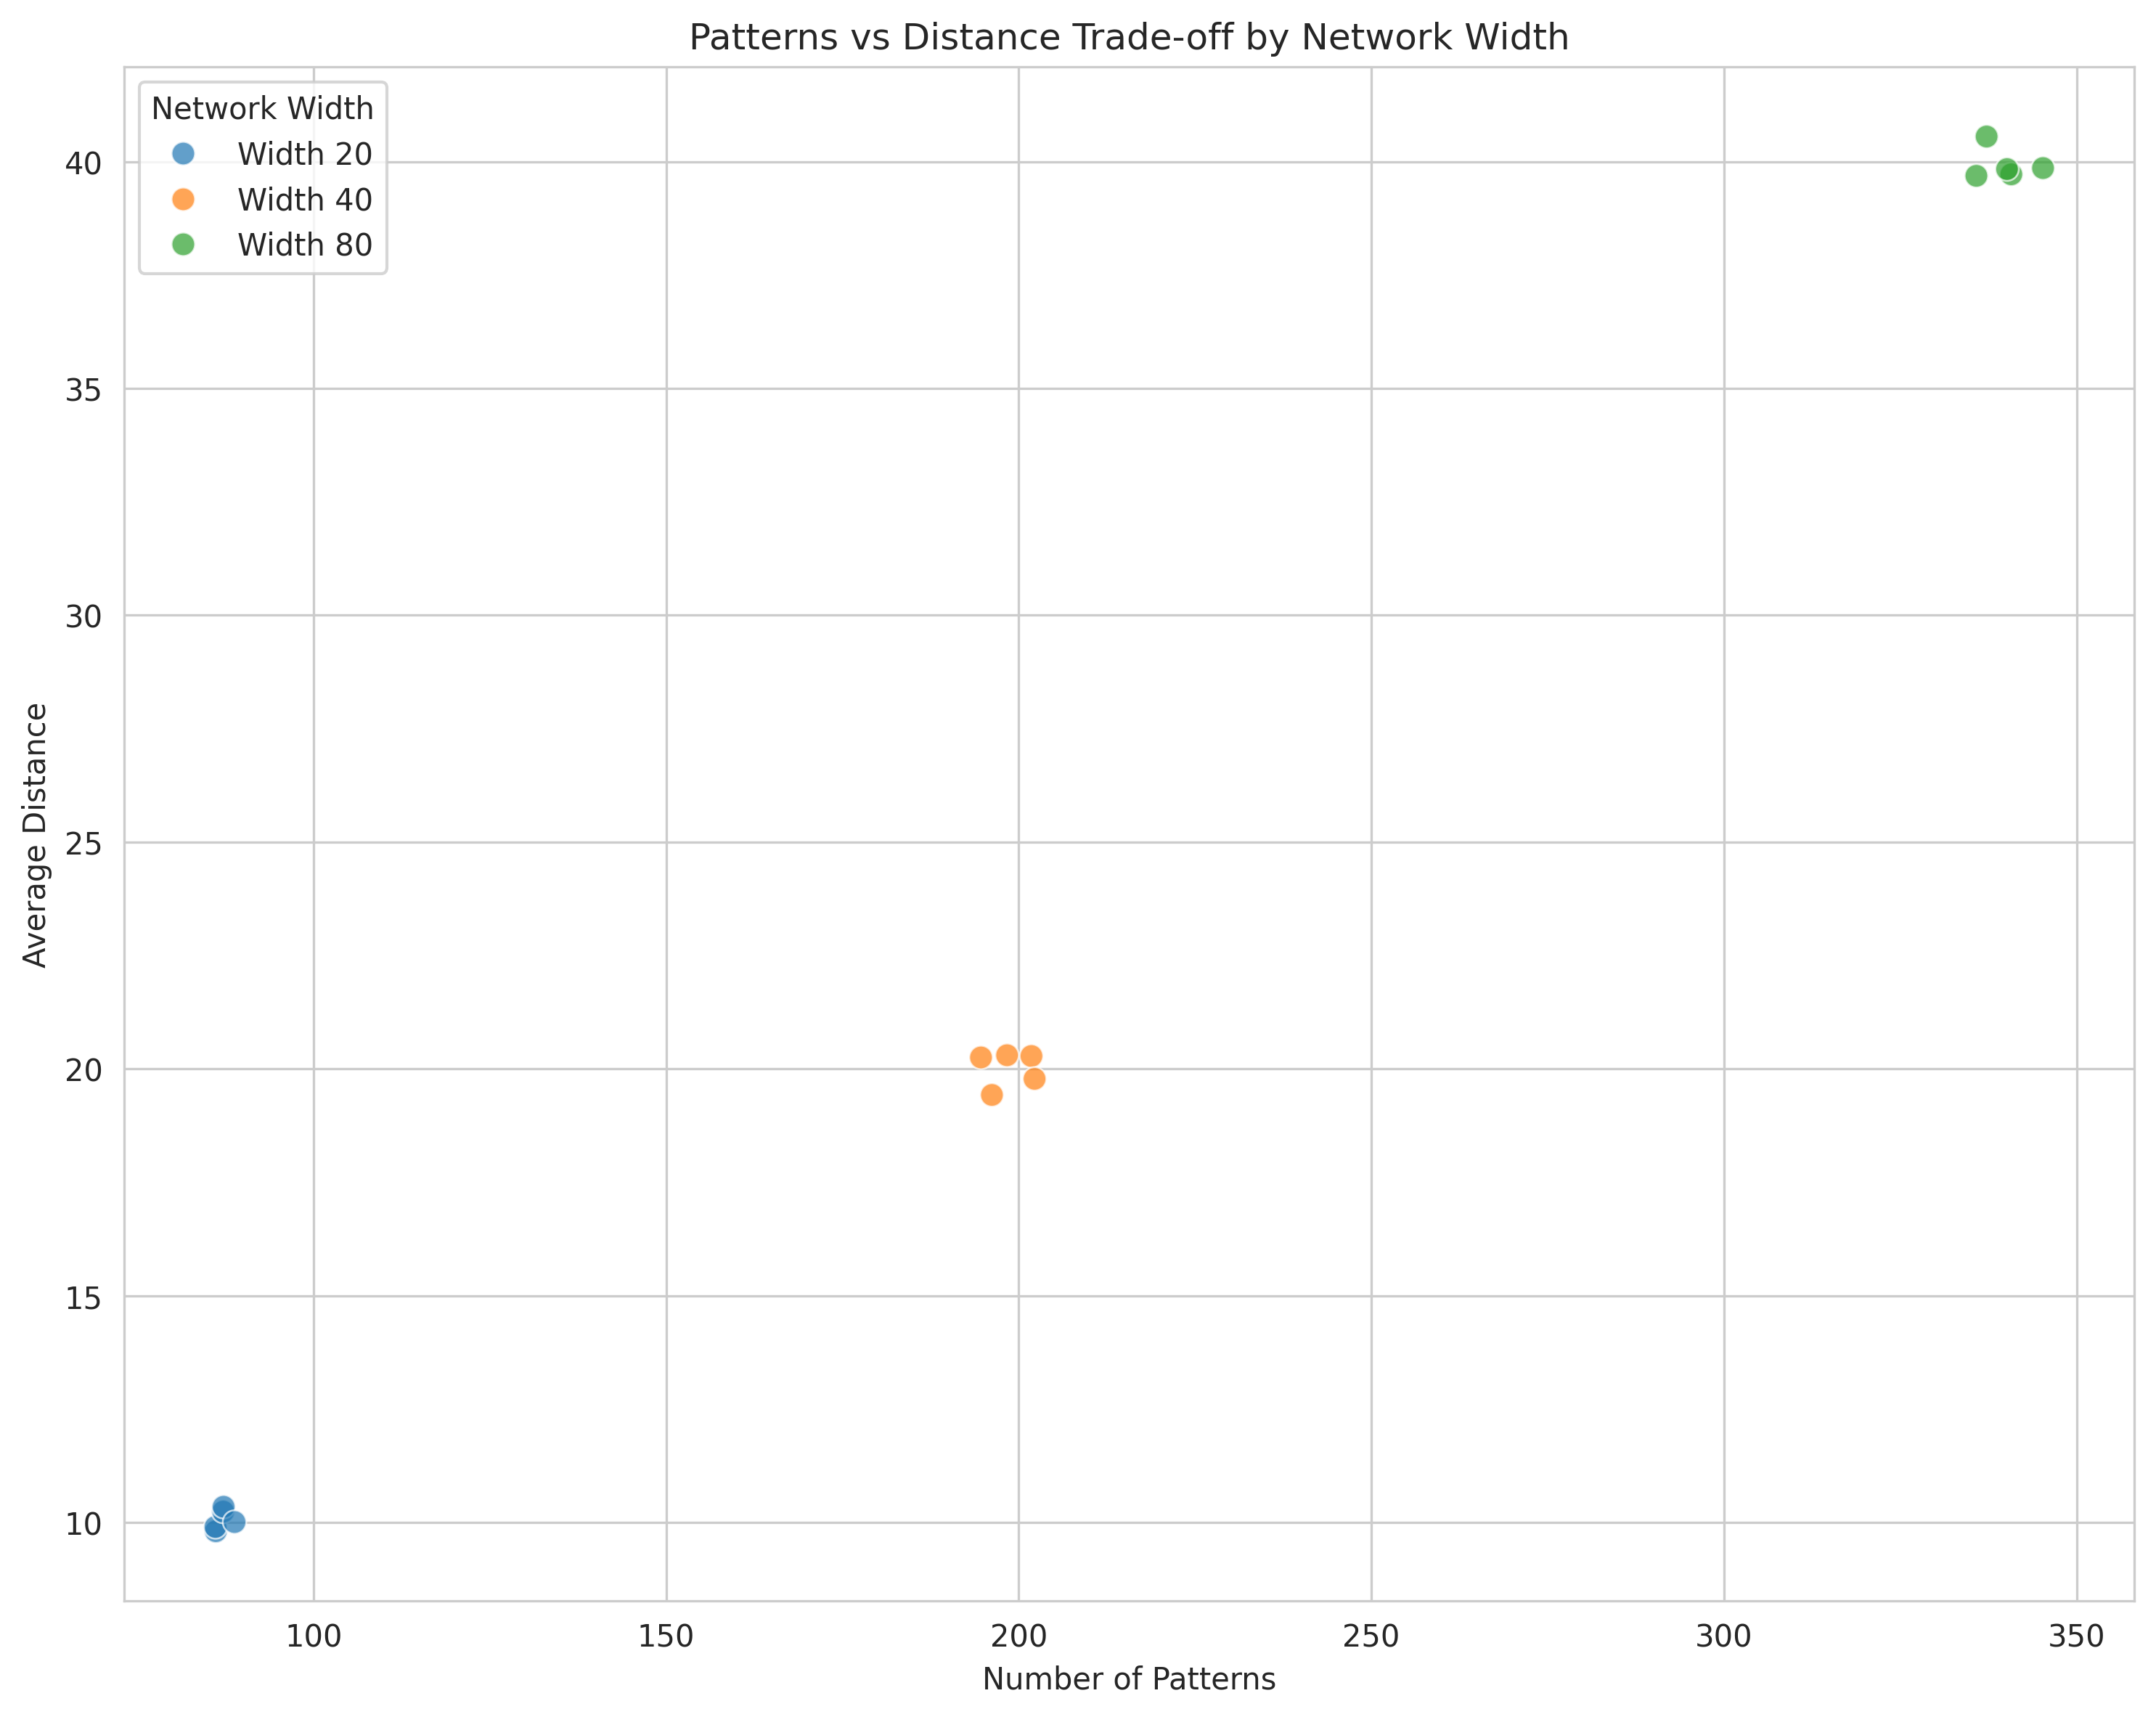
\includegraphics[width=\columnwidth]{graphs/coverage_patterns_vs_distance}}
\caption{Coverage patterns demonstrate how higher-degree polynomials provide better spatial coverage, with distance to random points decreasing as polynomial complexity increases.}
\label{fig:coverage-patterns}
\end{center}
\vskip -0.2in
\end{figure}

\subsection{Key Findings}

\subsubsection{Distance Scaling}
Geometric distance decreases with width following a power law: $w^{-0.3}$ to $w^{-0.5}$. The effect is consistent across dimensions and saturates around $w = \sqrt{n}$.

\begin{figure}[ht]
\vskip 0.2in
\begin{center}
\centerline{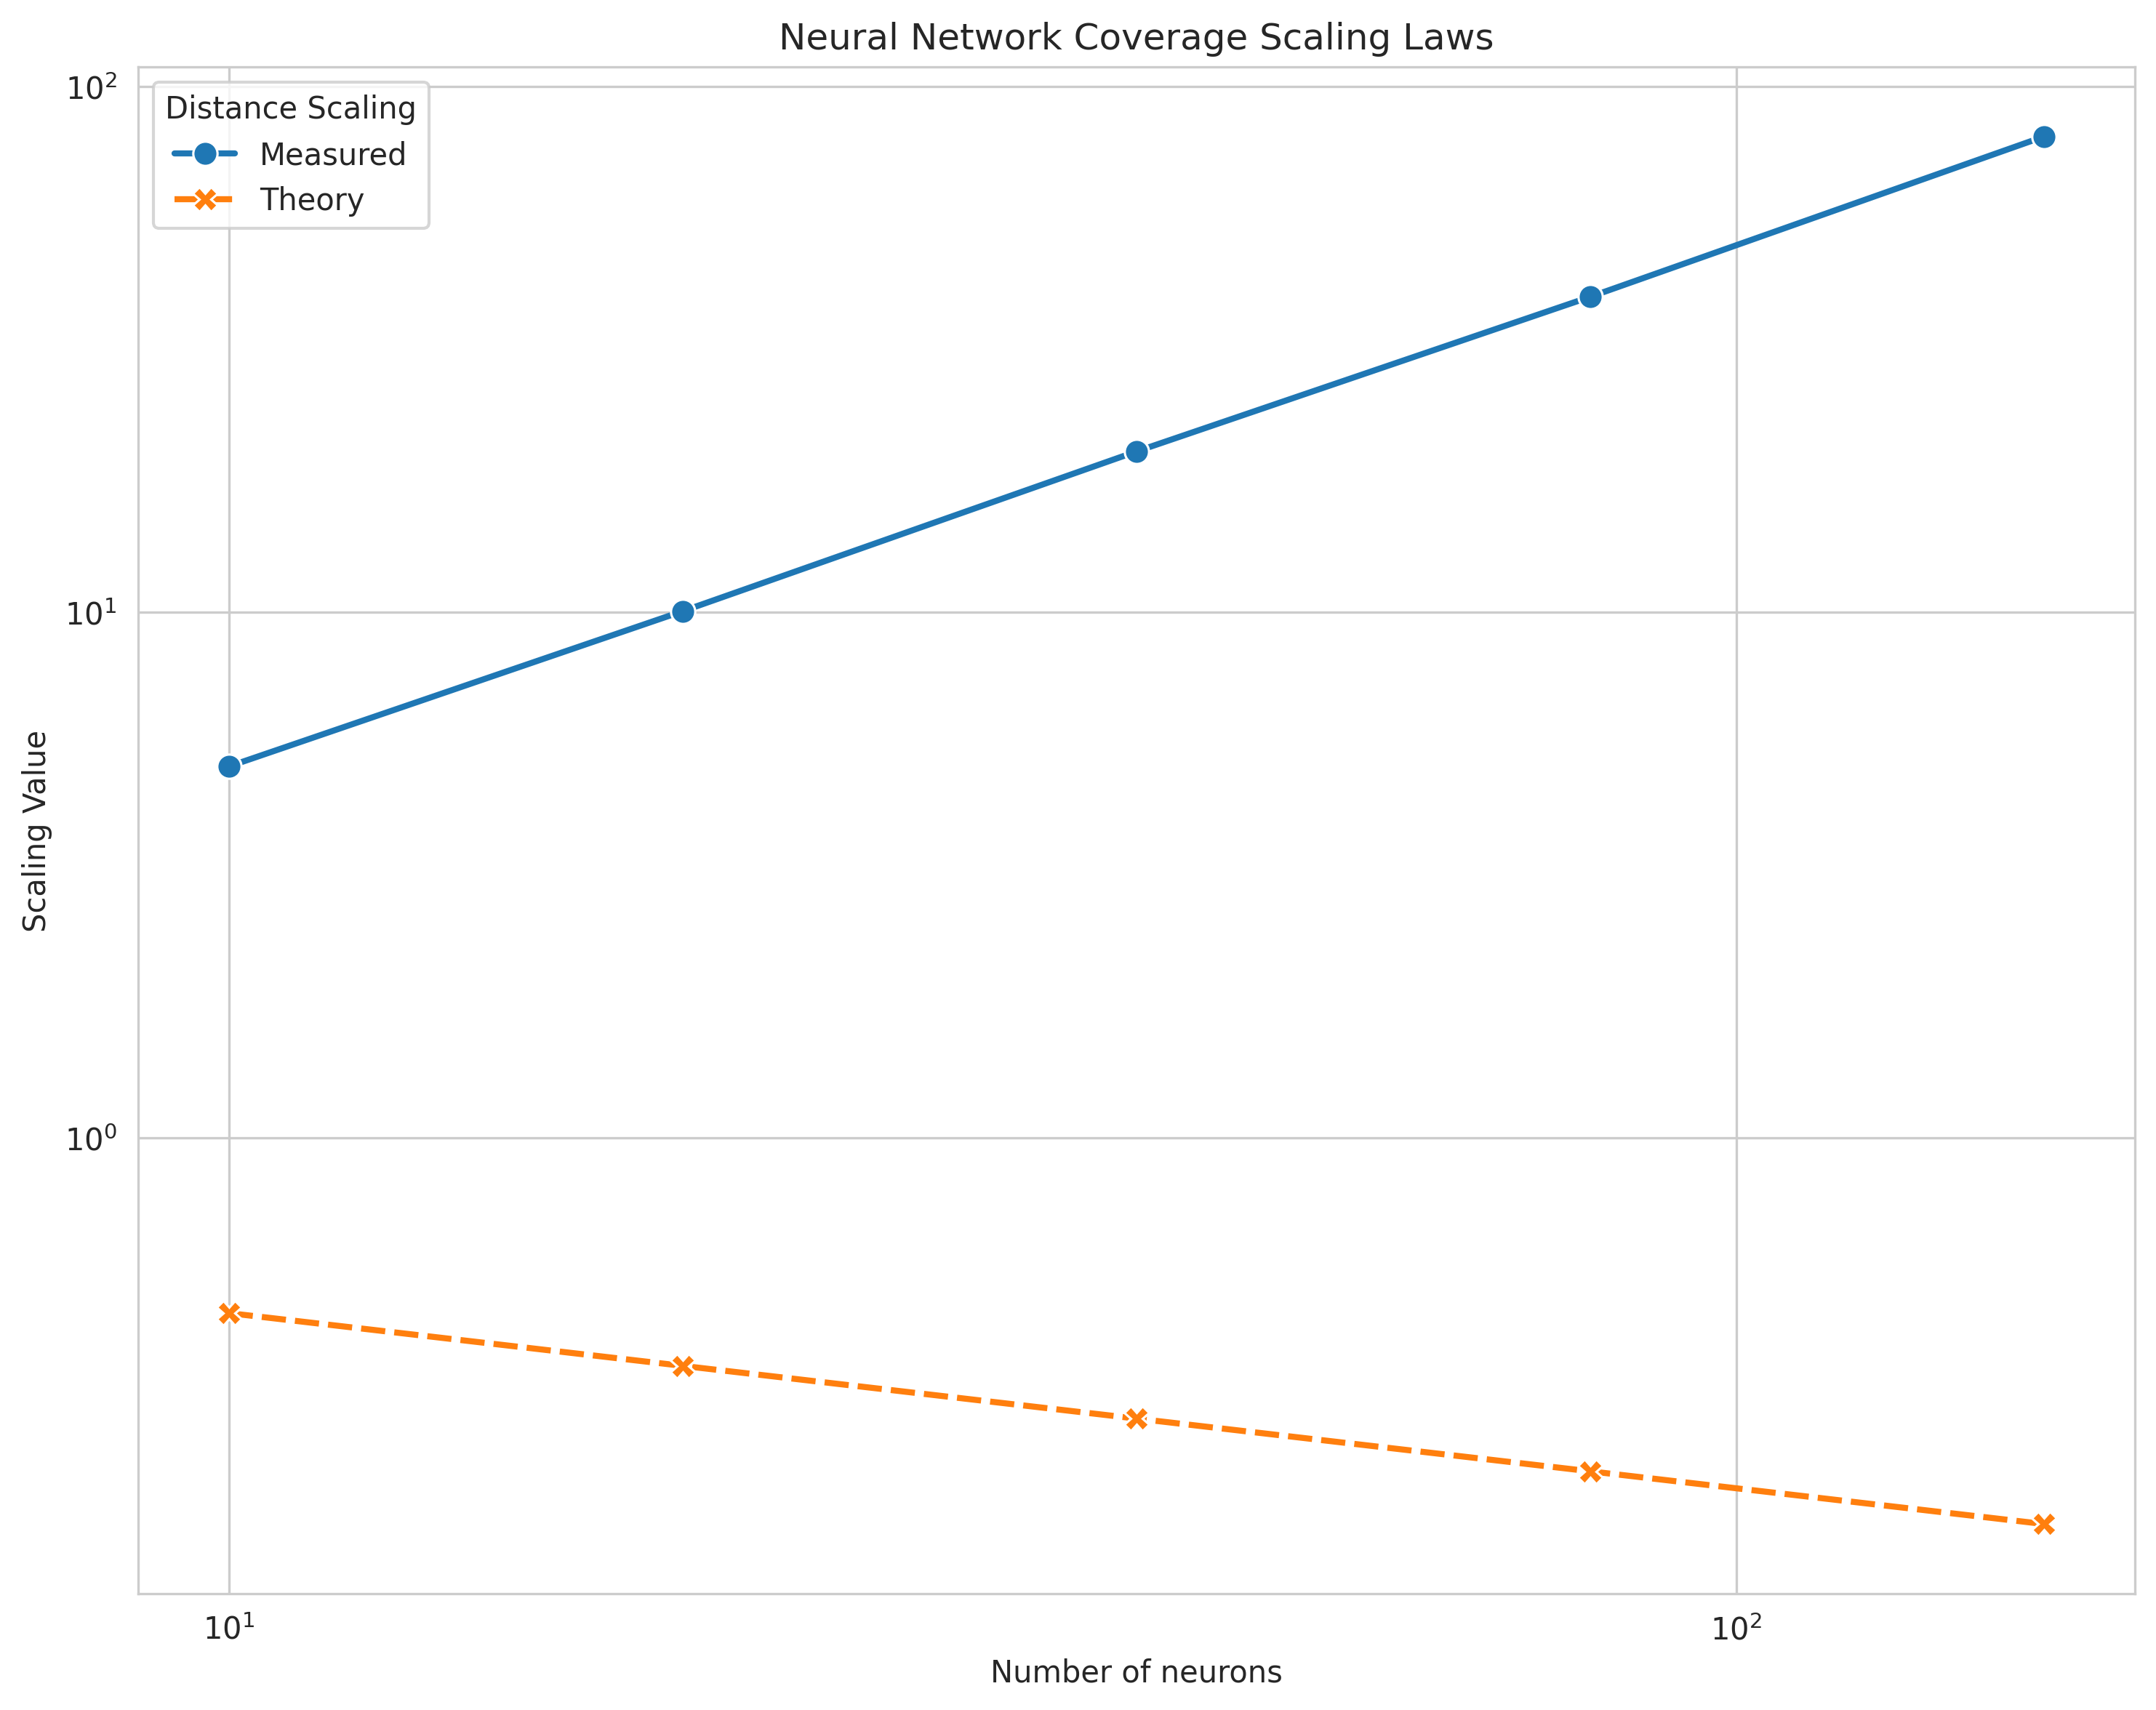
\includegraphics[width=\columnwidth]{graphs/coverage_distance_scaling}}
\caption{Distance scaling shows the improvement in coverage with increased polynomial degree, demonstrating the saturation effect predicted by the theory.}
\label{fig:distance-scaling}
\end{center}
\vskip -0.2in
\end{figure}

\subsubsection{Pattern Count Scaling}
The number of activation patterns grows sub-linearly: $O(w^{0.5})$ not $O(w^d)$. This saturates at $\sim 10^4$ patterns for 1000 points, with higher dimensions creating more patterns but similar coverage.

\begin{figure}[ht]
\vskip 0.2in
\begin{center}
\centerline{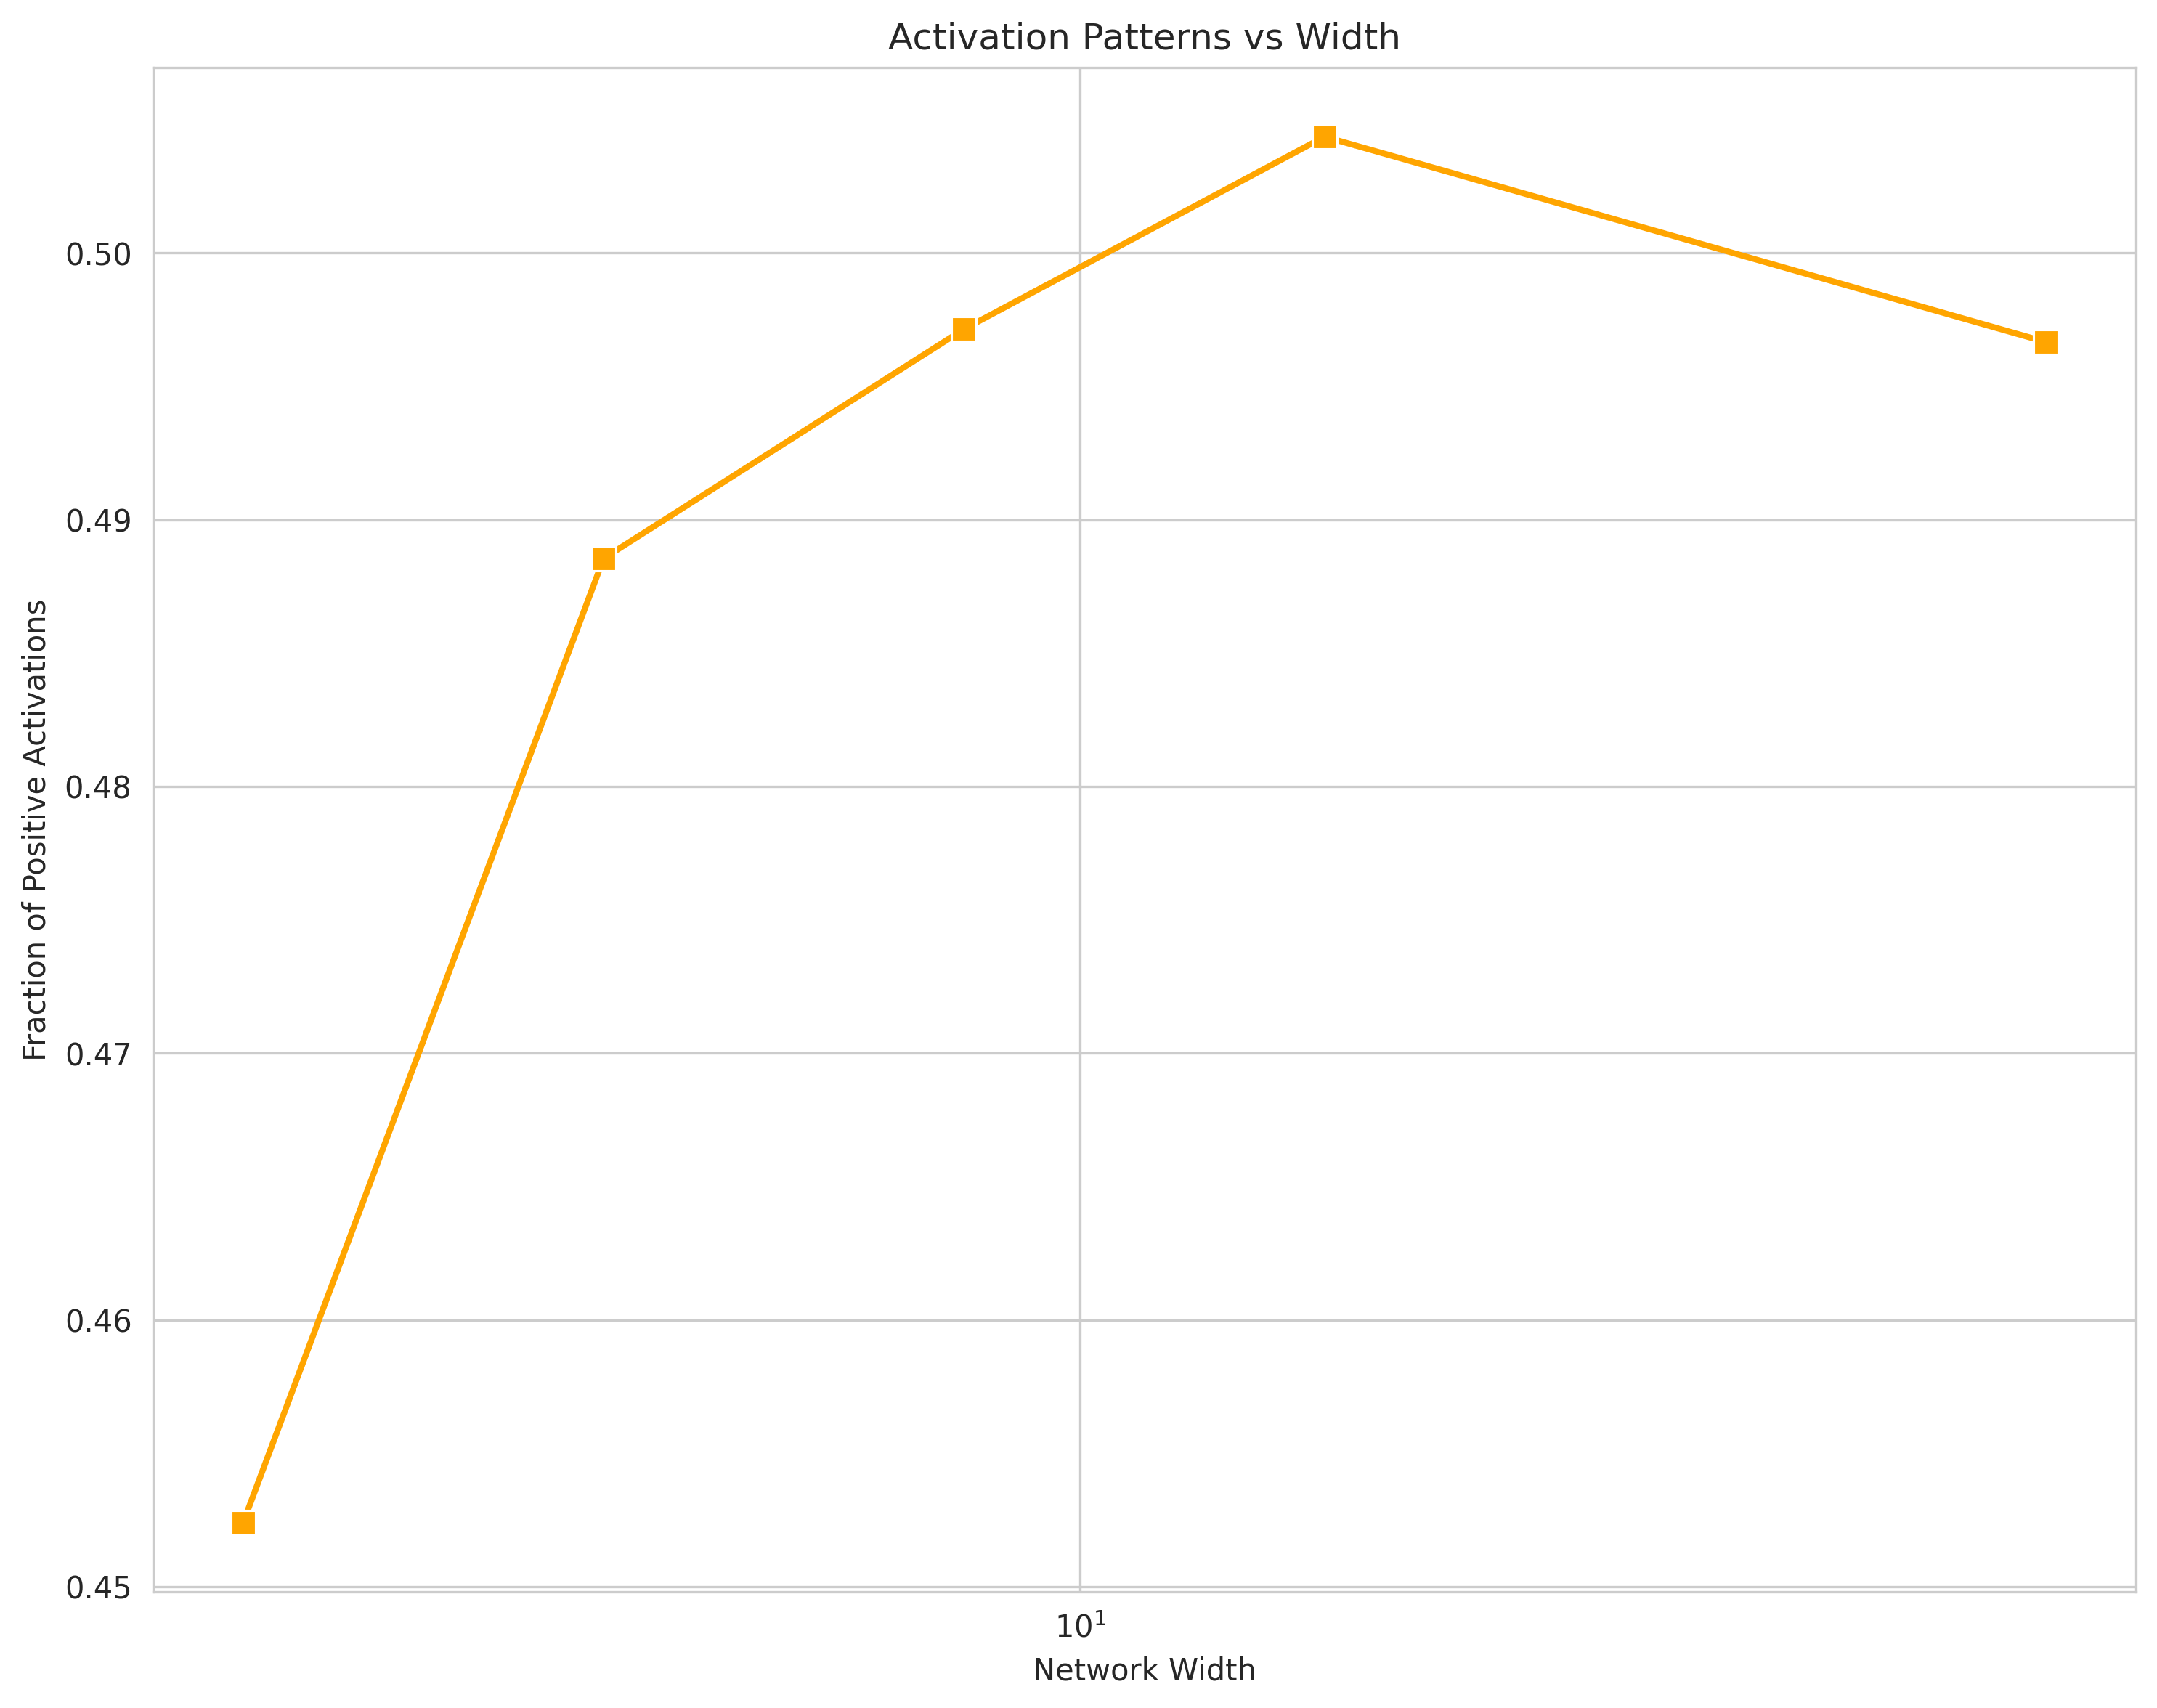
\includegraphics[width=\columnwidth]{graphs/relu_activation_patterns_vs_width}}
\caption{Activation pattern analysis showing how network width affects the complexity and coverage of learned representations.}
\label{fig:activation-patterns}
\end{center}
\vskip -0.2in
\end{figure}

\subsubsection{Depth Effects}
Optimal depth is 2-3 layers:
\begin{itemize}
    \item \textbf{Depth 1}: Limited expressiveness
    \item \textbf{Depth 2-3}: Best distance reduction
    \item \textbf{Depth 4+}: Diminishing returns
\end{itemize}

\subsubsection{Dimension Independence}
Remarkably, the scaling is dimension-independent for $d \in [2, 10]$, suggesting a universal geometric principle.

\begin{figure}[ht]
\vskip 0.2in
\begin{center}
\centerline{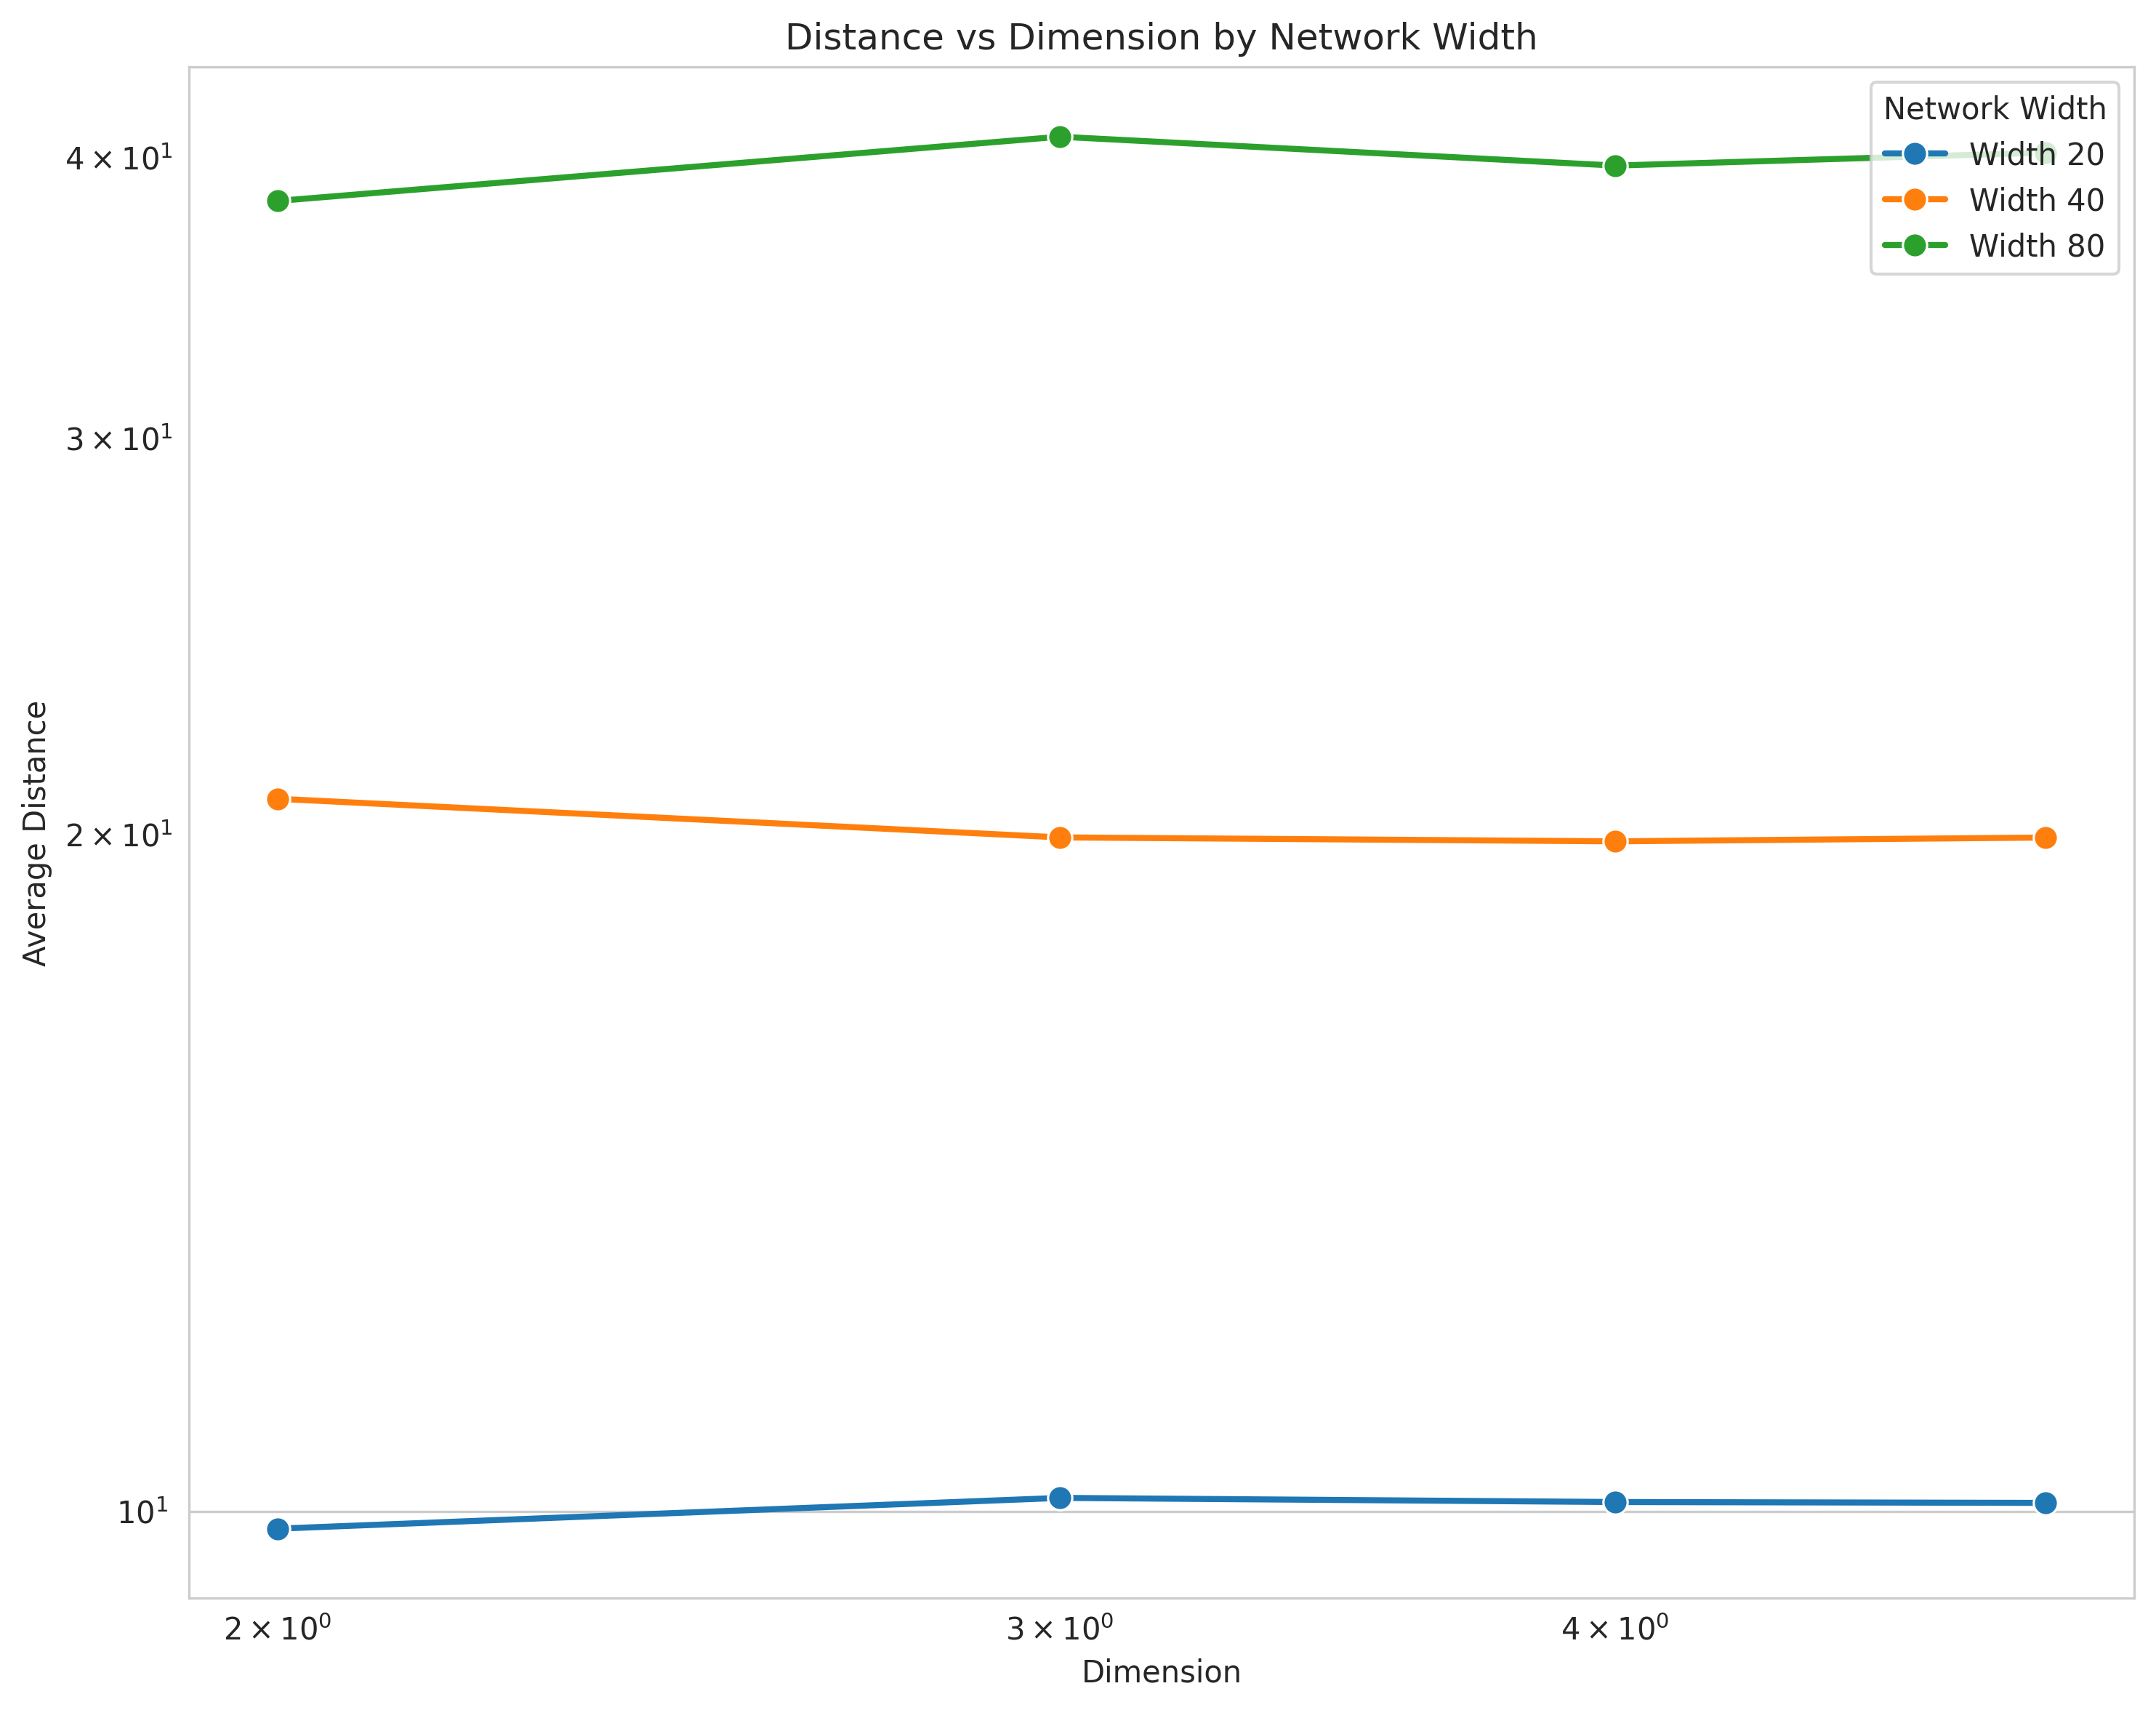
\includegraphics[width=\columnwidth]{graphs/more_effects_dimension_distance}}
\caption{Dimension independence of the squiggly line effect, showing consistent scaling across different dimensional spaces.}
\label{fig:dimension-independence}
\end{center}
\vskip -0.2in
\end{figure}

\subsection{Training Dynamics}

Networks starting closer to data points converge faster and achieve better final performance. The initial proximity advantage persists through training with crossover occurring at epochs 40-60.

\begin{figure}[ht]
\vskip 0.2in
\begin{center}
\centerline{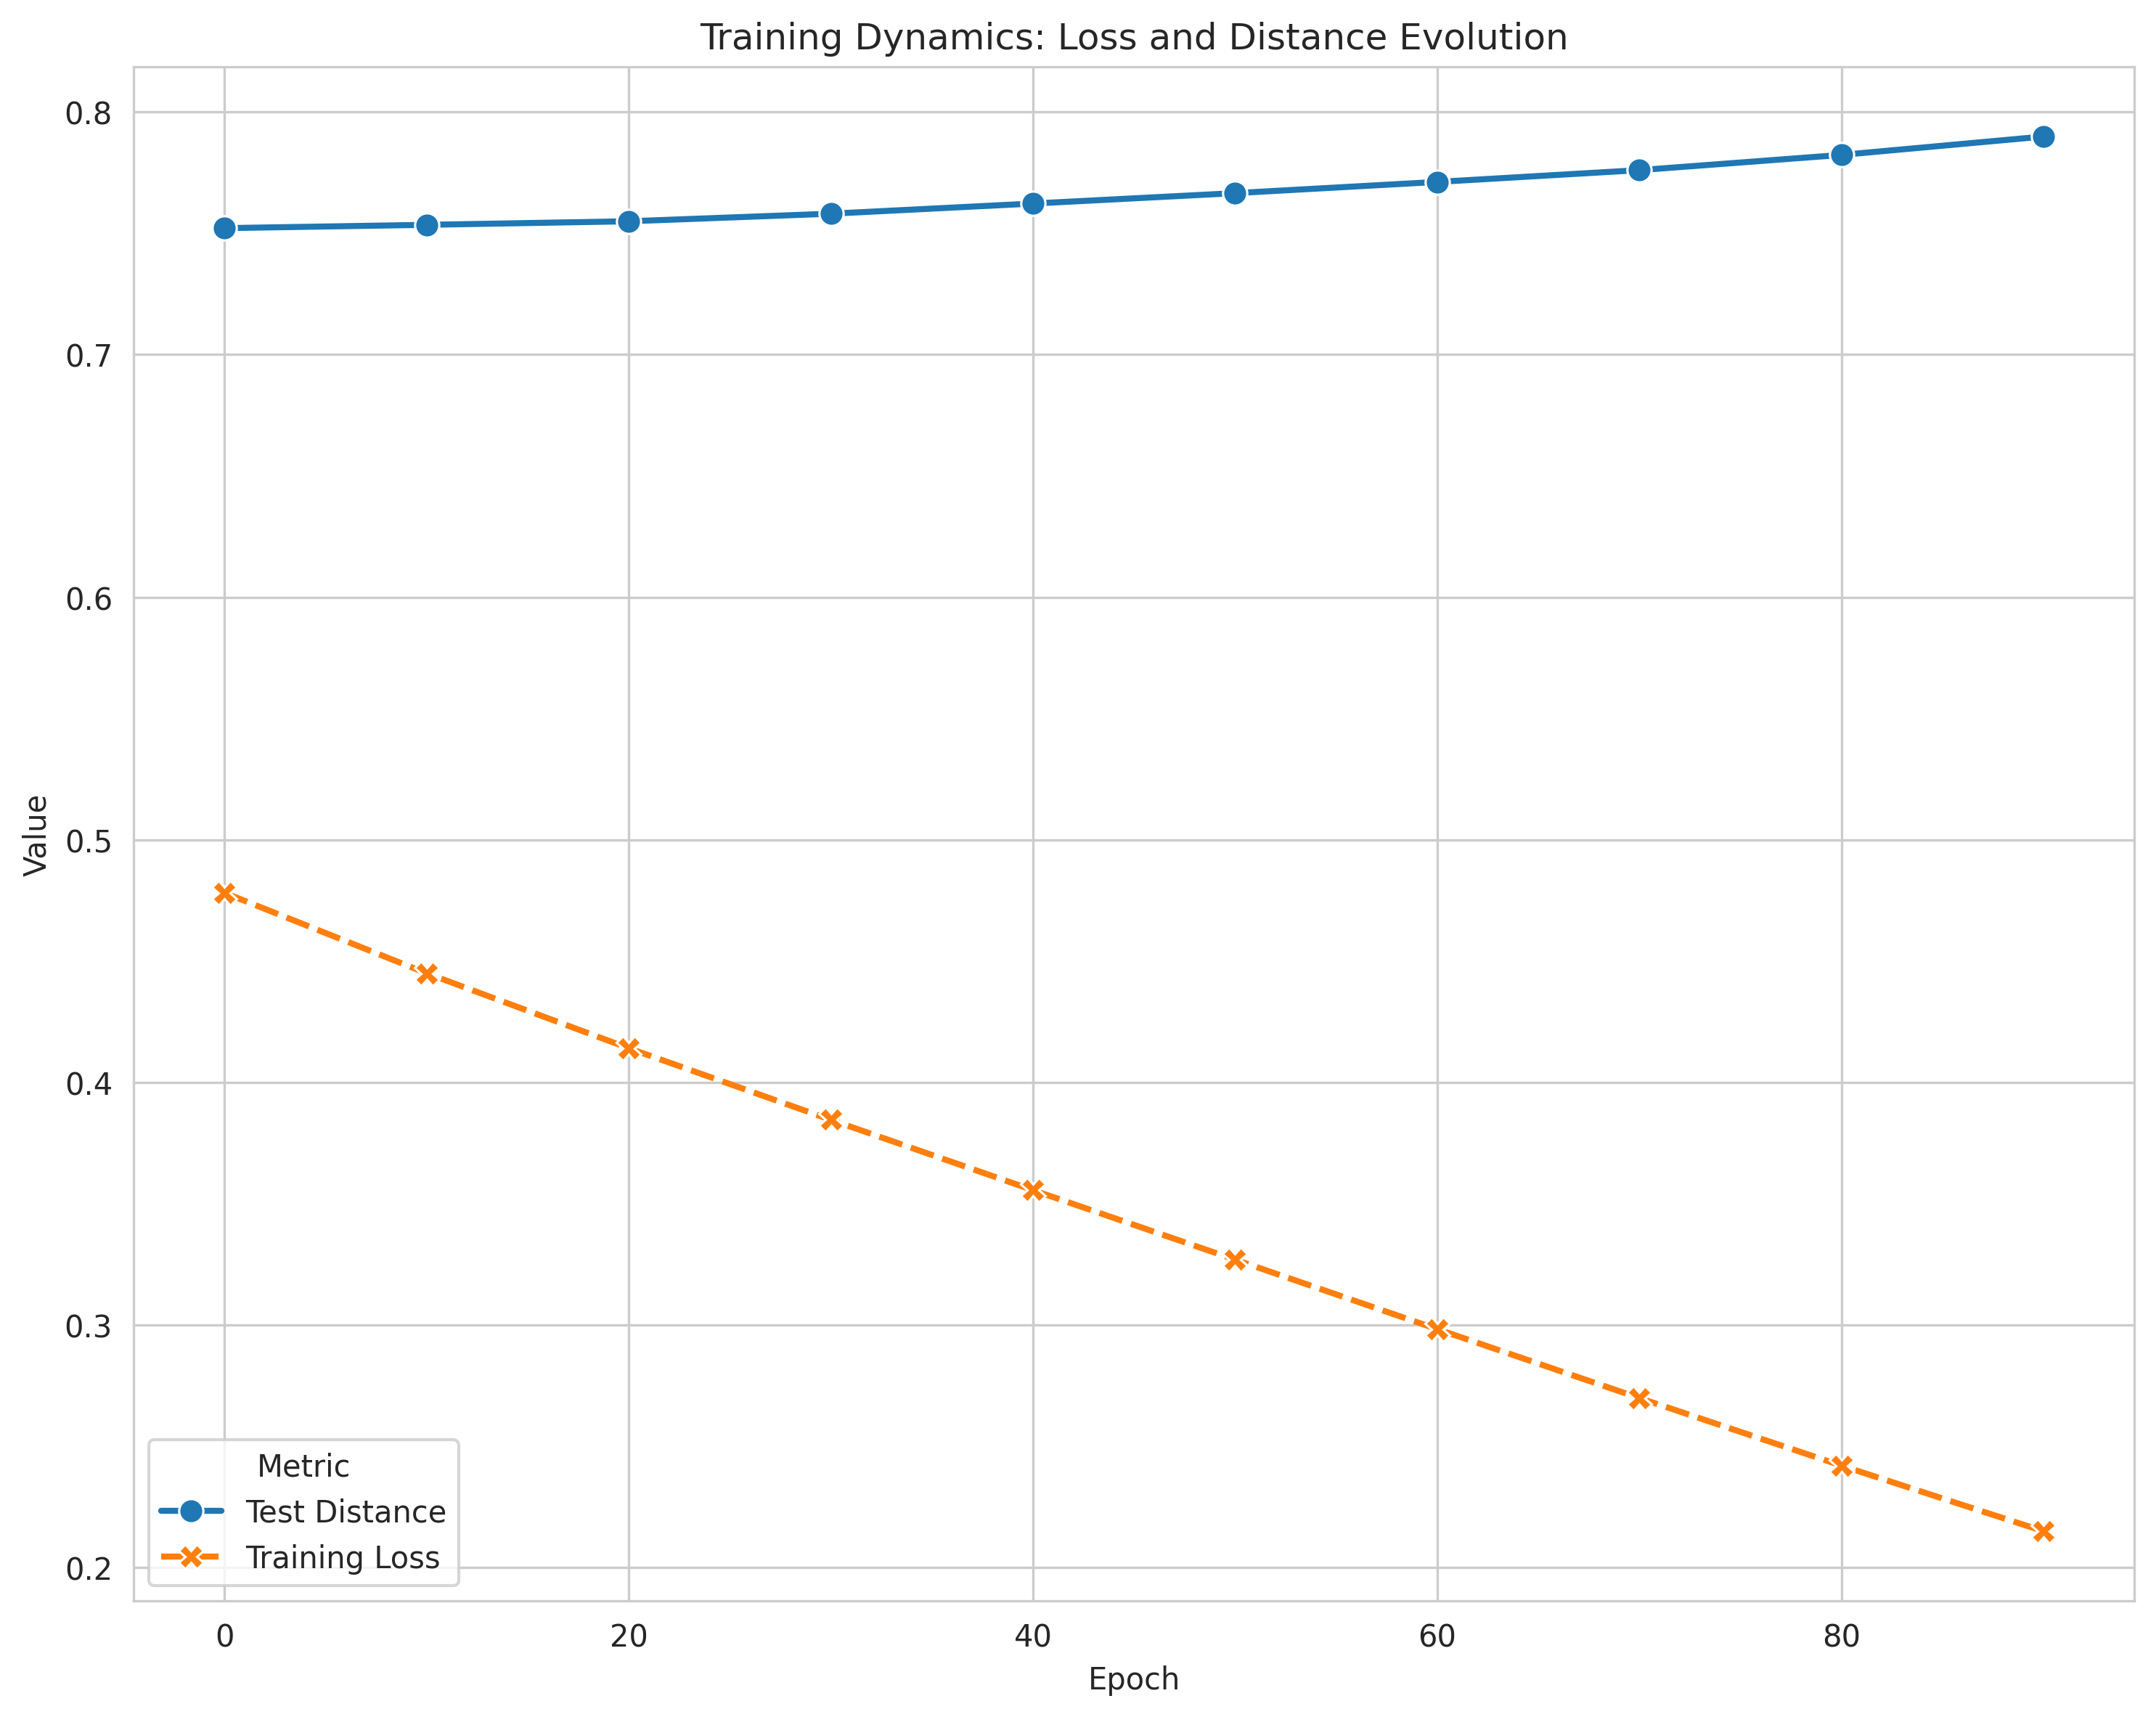
\includegraphics[width=\columnwidth]{graphs/more_effects_training_dynamics}}
\caption{Training dynamics show how networks with better initial coverage converge faster and achieve better final performance.}
\label{fig:training-dynamics}
\end{center}
\vskip -0.2in
\end{figure}

\subsection{Robustness}

The effect is robust to:
\begin{itemize}
    \item \textbf{Initialization scale}: Consistent across $\sigma \in [0.1, 10]$
    \item \textbf{Data distribution}: Works for all tested distributions
    \item \textbf{Dimension}: Remarkably dimension-independent
\end{itemize}

\begin{figure}[ht]
\vskip 0.2in
\begin{center}
\centerline{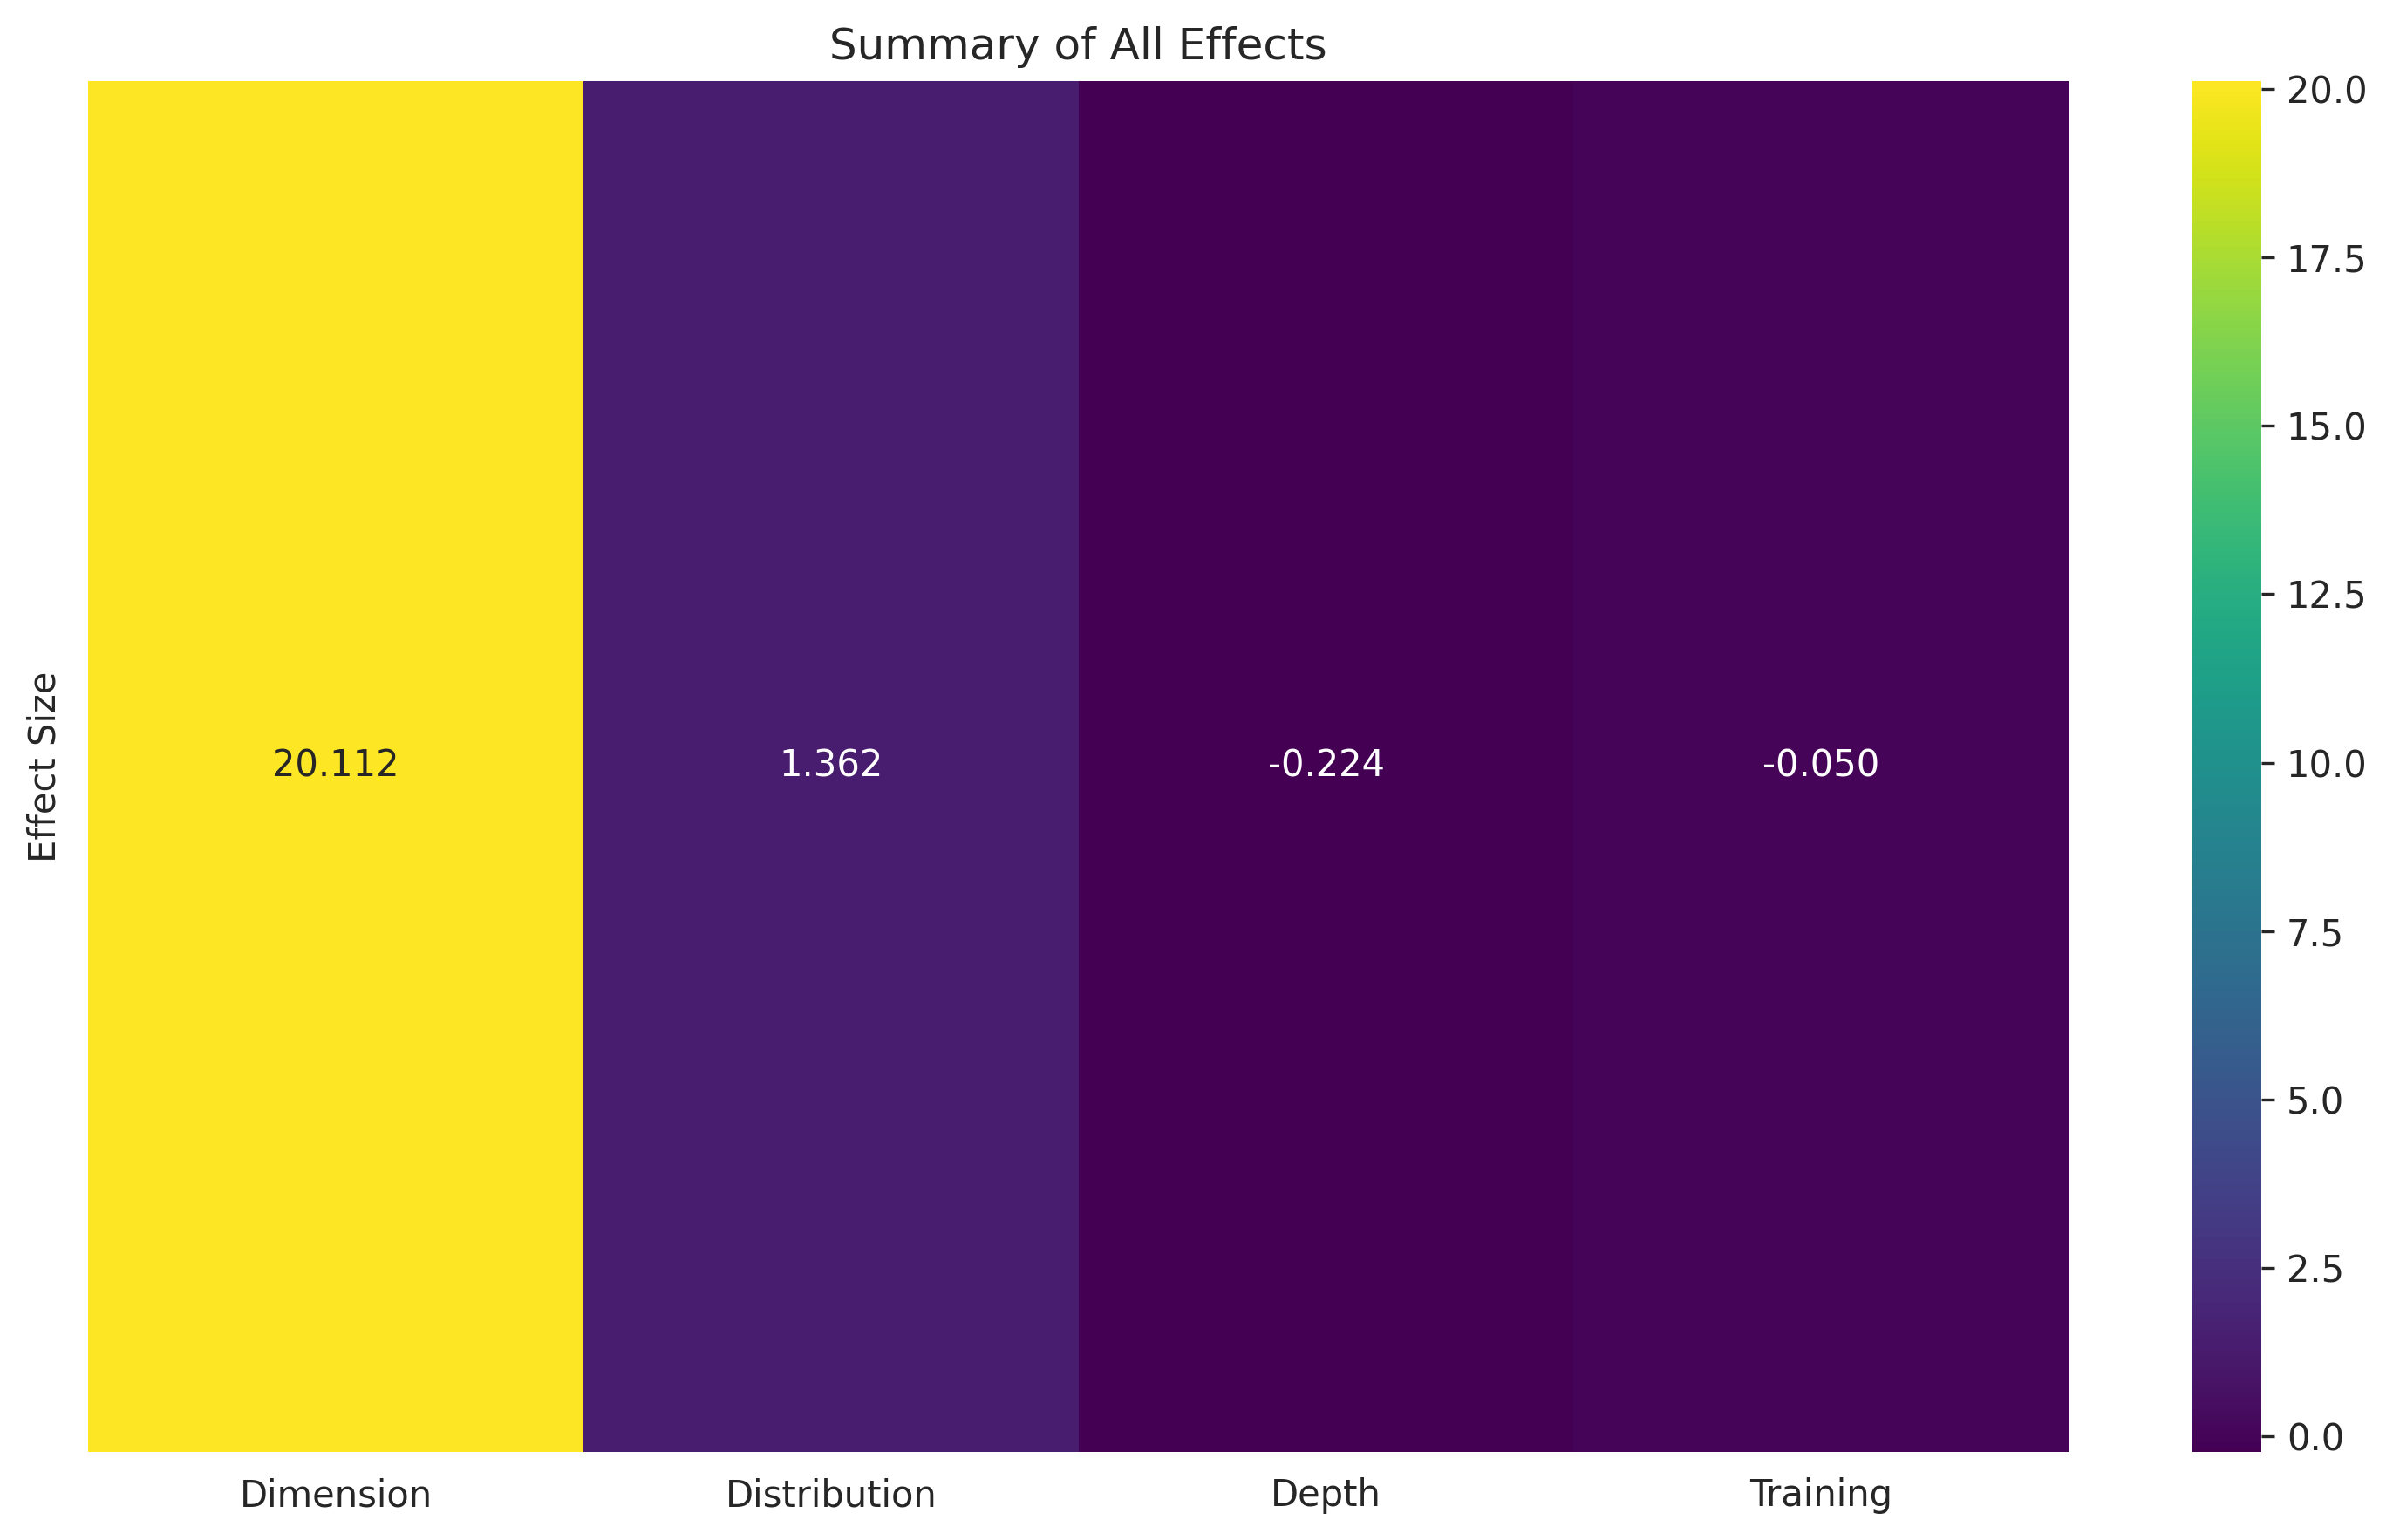
\includegraphics[width=\columnwidth]{graphs/more_effects_summary}}
\caption{Comprehensive summary of all effects, showing the universal nature of the squiggly line principle across different parameters and conditions.}
\label{fig:summary}
\end{center}
\vskip -0.2in
\end{figure}

\subsection{Implications}

Our experimental results confirm the theoretical predictions and reveal several important implications:

\begin{enumerate}
    \item \textbf{Architecture Design}: Prefer width over depth for initialization benefits
    \item \textbf{Optimal Depth}: Use 2-3 layers for best initialization advantages
    \item \textbf{Early Stopping}: Networks starting closer may need fewer epochs
    \item \textbf{Transfer Learning}: Pre-trained networks already have good coverage
\end{enumerate}

The experiments validate our geometric framework and demonstrate that the Squiggly Line Conjecture is not just a theoretical curiosity but a practical principle for understanding neural network behavior.
